\documentclass{article}
\usepackage{amsmath}
\usepackage{mathtools}
\usepackage{graphicx}
\title{The statistical problem of correlation as variational and eigenvalue problem, including its connection with the curve fitting\footnote{translated by Feng Zhao, the title of the original article is "Das statistische Problem der Korrelation als Variations- und Eigenwertproblem und sein Zusammenhang mit der Ausgleichsrechnung"}}

\date{December 2020}
\author{Hans Gebelein}

\begin{document}
\maketitle
\begin{centering}
A satisfied correlation metric is required to satisfy
the property that the two random variables are independent when the metric is zero and one is
determined by another when the metric is one.
The task to obtain such correlation metric is conducted
as a variational problem and can be transformed to solve
the smallest eigenvalue of a homogeneous Fredholm integral equation. By examining theses variational
problems we can obtain its relationship with the commonly used correlation metric and the curve fitting.
\end{centering}

\section{Problem formulation and commonly-used correlation metric}
One of the notable view for the judgement of two-dimensional probabilistic distribution $w(x,y)$ is by fixing one variable $x$, the distribution of $y$ is more or less influenced or not. As is well known,
Such influence does not exist when $w(x,y)$
is the product of a function $w_1(x)$ of $x$ and
a function $w_2(y)$ of $y$. $x$ and $y$
are mutually independent in such case. On the
other hand, it can happen that for each given $x$
only a single $y$ is corresponded. Then $y$
is a function of $x$ and we say a complete correlation
exists between the two variables. In general the result lies between the two extreme cases, and there is a question about a metric for the tightness of the relationship
between $x$ and $y$. This is the correlation problem of statistics.

To characterize the correlation between $y$ and $x$,
there are many well-known different metrics, which we firstly quote here. Especially we observe a so-called
geometric probabilistic distribution for the random variable $x$ and $y$. Such pair is determined by the
positive function $w(x,y)$ by the normalization condition:
\begin{equation}\label{eq:wxy}
    \iint w(x,y) dx dy = 1
\end{equation}
Integrating by $x$ or $y$ we can obtain
\begin{equation}\label{eq:w12}
    w_1(x) = \int w(x,y)dy \textrm{ and }
    w_2(y) = \int w(x,y)dx
\end{equation}
Their integral about $x$ or $y$ is 1. In the following we use $a$
and $b$ to describe the mean value of $x$ and $y$
with respect to the distribution $w(x,y)$.
This is the center or mass coordinate of the mass
density on the $xy$-plane. It is
\begin{align}
    a = \iint x w(x,y) dx dy = \int x w_1(x)dx \notag \\
    b = \iint y w(x,y) dx dy = \int y w_2(y)dy \label{eq:ab}
\end{align}
Further $s^2$ and $t^2$ mean the stastical dispersion of $x$ around its mean value $a$
or $y$ around its mean value $b$ respectively.
These are moment of inertia of the plane with $w(x,y)$ as the density around the axis through the
center of mass and parallel to the coordinate axis. It is defined as:
\begin{align}
    s^2 = \iint (x-a)^2 w(x,y) dx dy = \int (x-a)^2 w_1(x)dx \notag \\
    t^2 = \iint (y-b)^2 w(x,y) dx dy = \int (y-b)^2 w_2(y)dy 
    \label{eq:st}
\end{align}
As the correlation metric we need consider a numerical quantity, which should satisfy three properties.
Firstly it can be computed from any given two-parameter distribution. Secondly the value should
be zero is $x$ and $y$ are statistically independent. Thirdly the value should be one is $x$ and $y$
are fully dependent.

The classtical correlation coefficient satisfies the first and second condition, which is based on the moment of deviation
of the distribution:
\begin{equation}
r = \frac{1}{st} \iint (x-a)(y-b)w(x,y)dxdy
\end{equation}
We always have $r^2 \leq 1$.
The value $r=+ 1$ occurs when $y$ has positive linear relationship with $x$.
The value $r= - 1$ occurs when $y$ has negative linear relationship with $x$.
The disadvantage of this correlation coefficient is that based on $r=0$ we cannot get the
full independence condition $w(x,y)=w_1(x)w_2(y)$.
On the other hand, when $x$ and $y$ have full statistical non-linear dependence, $r$
is different from one.

To remedy the second shortcoming other correlation metrics are proposed.
A unified method to the detailed analysis of the distribution $w(x,y)$ are the regression line $\bar{y}(x)$ and $\bar{x}(y)$.
They are the mechanical view of the geometric place for the center of mass of the strip in
the $xy$-plane parallel to the coordinate axes.
\begin{align}
   \bar{y}(x) = \frac{\int y w(x,y) dy}{\int w(x,y) dy} = \frac{1}{w_1(x)} \int y w(x, y)dy \notag \\
   \bar{x}(y) =  \frac{\int x w(x,y) dx}{\int w(x,y) dx} = \frac{1}{w_2(x)} \int x w(x, y)dx  \label{eq:barxy}
\end{align}
In the two extreme cases of statistical independence and
full dependence, the two regression lines are clearly
characterized. For independence we have $\bar{y}(x) = b$
and $\bar{x}(y)=a$ due to $w(x,y) = w_1(x)w_2(y)$.
That is, the regression lines are the horizontal and
the vertical straight lines through the center of mass of the
distribution. It should be noted that from this condition of regression lines,
the center of mass cannot be inferred reversely based on the assumption of statistical independence.
Actually we cannot deduce $w(x,y)=w_1(x)w_2(y)$.

On the other hand, under
the condition of full dependence, $x$ and
$y$ are determined by the function $y(x)$
and $x(y)$ explicitly. We have $\bar{y}(x) = y(x)$
and $\bar{x}(y) = x(y)$ so that in this case
the two regression lines coincide.

In statistical practice, based on the regression lines,
Pearson introduced \textsf{correlation ratio}.
\begin{align}
   k^2_{yx} = \frac{1}{t^2}\int (\bar{y}(x) - b)^2 w_1(x)dx \textrm{ (correlation ratio of $y$ to $x$}) \notag \\
   k^2_{xy} = \frac{1}{s^2}\int (\bar{x}(y) - a)^2 w_2(y)dy \textrm{ (correlation ratio of $y$ to $x$}) \label{eq:pr}
\end{align}
These correlation ratio take value zero at independence
condition and in particular take value one at full
dependence condition. Therefore, the measure of correlation with the help of this quantity is very satisfied when they are equal. If we are not dealing with the two extreme
cases with $k^2_{yx} = k^2_{xy}=0$ or $1$, then
generally $k^2_{yx}$ is not equal to $k^2_{xy}$. Only when the regression lines are straight, the two correlation coefficients take the same value, and this
value also equal to the square of the correlation
coefficient $r$.

Pearson also suggested another measure of correlation metric as \textsf{Mean square Contingency}.
\begin{align}
   f^2 &= \frac{1}{\sqrt{(m-1)(n-1)}}\sum_{ik}
   \frac{(w(x_i,y_k)-w_1(x_i)w_2(y_k))^2}{w_1(x_i)w_2(y_k)} \notag \\
   &=\frac{1}{\sqrt{(m-1)(n-1)}}\left(\sum_{ik}
   \frac{w^2(x_i,y_k)}{w_1(x_i)w_2(y_k)} -1\right)
\end{align}
Here the discrete distribution must be assumed, in
which $m$ and $n$ are the number of rows and columns of the so-called correlation table. Then
under the condition of statistical independence $w(x_i,y_k) = w_1(x_i)w_2(y_k)$, $f^2=0$ is obvious.
Under the condition of full dependence, $m=n$ is necessary. $w(x_i,y_k)$ has only $n$ non-zero
probability values
$$
w(x_i, y_k) = w_1(x_i) = w_2(y_k)
$$
Then there are $n$ non-zero terms $w^2(x_i, y_k)/w_1(x_i)w_2(y_k)$, which are all one, and due
to $m=n$ we have $f^2=1$.

The particular advantage of this correlation metric
of Pearson is that the value depends only on the
frequency, not on the value of $x$ or $y$.
Hence this metric also allows other non-numerical
quantities like color, gender etc. Its disadvantage is
that $f^2$ is defined only for the discrete distribution and we will show later that the natural generalization to $w(x,y)$ is not possible in general.

All these existing correlation metrics have special
advantages and disadvantages. Their relationship with
each other is not easily observed. In the following
we show that the correlation problem can be formulated
as a variational problem, and this variational problem
can be transformed to the homogeneous Fredholm integral equation, where we can solve the eigenvalue problem.
We find that the commonly used correlation metrics are not others but different method to approximate the smallest eigenvalue of this integral equation.
If we are dealing with a discrete distribution, then the integral equation degenerates to a homogeneous linear equation system.

The question about the best relation between $y$ and
$x$ is also met in curve fitting, which deals with
a sequence of observed points by finding a simple curve
to best fit the data. We deal with the curve fitting problem by treating it as a correlation problem, which provides new point of view for the solution. It shows that from correlation problem, we can develop good methods to solve the task of curve fitting.
\section{Variational problem and integral equation}
All the existing correlation metrics have certain shortcomings. Without consideration of calculability, now we ask the question about a theoretical perfect and conceptual simple correlation metric.
With respect to the conceptual simplicity, the correlation coefficient is the most satisfying.
Its main disadvantage is that under non-linear transformation of the random variable $x$
and $y$, the quantity is not invariant.
If the two quantities are assigned other values,
that is, if $x$ is transformed by $f(x)$ and $y$
is transformed by $g(y)$, then the value of $r$
varies in general. The disadvantage of the quantity $r$
is removed when all these kinds of transformations
are considered. To obtain an improved correlation metric,
we inquire for the greatest value which $r$ can achieve by
such transformation. Then we have the following variational problem:

Given a positive function $w(x,y)$ which satisfies the
normalization condition $\iint w(x,y)dxdy=1$. It is to determine the function $f(x)$ and $g(y)$ such that
\begin{equation}
    K^2 = \max\frac{(\iint f(x)g(y)w(x,y)dxdy)^2}
    {\iint f^2(x)w(x,y)dxdy \iint g^(y) w(x,y)dxdy}
\end{equation}
Then $K^2$ is a measure for the correlation of the distribution
$w(x,y)$. In the term of mechanics,
the correlation measure is the largest value of the quotient
of the moment of deviation divided by the two moments of inertia for the distribution when all kinds of distortion in $x$ or $y$ direction are allowed.

We can write the variational problem in a simpler way when 
only normalized functions $f(x)$ and $g(y)$ are allowed.
That is:
\begin{align}
\iint f^2(x) w(x,y)dxdy &= \iint f^2(x)w_1(x)dx=1\notag\\
\iint g^2(x) w(x,y)dxdy &= \iint g^2(x)w_2(y)dy=1 \label{eq:fgw}
\end{align}
Functions like $f(x)=1, f(x)=\frac{x-a}{s}$
and $g(y)=1, g(y)=\frac{y-b}{t}$ satisfy \eqref{eq:fgw}
where $a,b,s,t$ are defined in (\ref{eq:ab}, \ref{eq:st}).
Owing to this constraint the variational problem of correlation becomes:
\begin{equation}\label{eq:K2}
    K^2 = (\max \iint f(x)g(y)dxdy)^2
\end{equation}
To guarantee this variational problem meaningful, another
side condition is necessary. Since $w(x,y)\geq 0$, by
Cauchy-Schwarz inequality
\begin{align*}
    (\iint f(x)g(y)w(x,y)dxdy)^2
    &= (\iint f(x)\sqrt{w(x,y)} \cdot g(y)\sqrt{w(x,y)}dxdy)^2\\
    &\le \iint f^2(x)w(x,y)dxdy\cdot 
    \iint g^2(x)w(x,y)dxdy = 1
\end{align*}
From this estimation the equality holds when the function
$f(x)\sqrt{w(x,y)}$ and $g(y)\sqrt{w(x,y)}$ are proportional.
This holds for any $w(x,y)$ when $f(x)=g(y)=1$. This case is trivial from \eqref{eq:wxy} and should be excluded. Therefore, for the variational problem we only allow
functions which are orthogonal to $f(x)=1$ (or $g(y)=1$)
with respect to $w_1(x)$ (or $w_2(y)$). This condition goes
as
\begin{align}
    \iint f(x)w(x,y)dxdy = \int f(x)w_1(x)dx=0 \notag\\
        \iint g(x)w(x,y)dxdy = \int g(y)w_2(y)dy=0
        \label{eq:fwgw0}
\end{align}
If this condition is fulfilled, $K^2$ is strictly less than
one in general. In particular in the case of full
statistical dependence due to $w(x,y)=w_1(x)w_2(y)$
$$
\iint f(x)g(y) w(x,y) dxdy=
\int f(x)w_1(x)dx \int g(y) w_2(y) dy = 0
$$
we have $K^2=0$.

According to (\ref{eq:ab}, \ref{eq:st}), the functions
$f(x) = \frac{x-a}{s}$
and $g(y) = \frac{y-b}{t}$
satisfy the condition \eqref{eq:fwgw0}.
Using these functions in \eqref{eq:K2},
we can get the correlation coefficient $r$. Therefore the
following estimation holds:
\begin{equation}
    r^2 \leq K^2 \leq 1
\end{equation}
To make sure the above result holds, the correlation
coefficient $r$ is no more than one for any distribution
$w(x,y)$.

The variational problem \eqref{eq:K2} 
contains two available functions.
We proceed with such case with only one free function,
in which we firstly treat $f(x)$ or $g(y)$ fix and determine
the other function such that the double intergral takes the largest
value. The task can be solved by applying Cauchy-Schwarz
inequality $(\int FGdx)^2 \leq \int F^2dx \int G^2dx$ where
$$
F(x)=f(x)\sqrt{w_1(x)},
G(x)=\frac{1}{\sqrt{w_1(x)}}\int g(y) w(x,y)dy
$$
Then we have
\begin{align*}
    (\iint f(x)g(y) w(x,y) dxdy)^2
    &= \left(\int f(x)\sqrt{w_1(x)} \cdot (\frac{1}{\sqrt{w_1(x)}}
    \int g(y)w(x,y)dy) dx\right)^2 \\
    &\leq \int \underbrace{f^2(x) w_1(x) dx}_{=1} \cdot
    \int \frac{1}{w_1(x)} (\int g(y) w(x,y)dy)^2 dx \\
    &= \int \frac{1}{w_1(x)} (\int g(y) w(x,y)dy)^2 dx
\end{align*}
This is the largest value that the variational
integral can take for a determined $g(y)$ and arbitrary
$f(x)$. The upper bound is reached when $F(x)$ and $G(x)$ are proportional to each other, or $f(x)$ and $g(x)$ satisfy
the equation
\begin{align*}
    \frac{G(x)}{F(x)}
    = \frac{\int g(y) w(x,y)dy}{w_1(x)f(x)}
    = \textrm{const.} = C
\end{align*}
The constant $C$ is obtained
by integration on both side of equation $C^2F^2(x) = G^2(x)$.
Since $\int F^2(x) x = 1$, we obtain
$$
C^2 = \int G^2(x)dx
= \int \frac{1}{w_1(x)} (\int g(y) w(x,y)dy)^2 dx
$$
which is exactly the value of the upper bound in the
estimation.

Therefore we obtain the result: Let $g(y)$ fixed and 
the function $f(x)$ is changeable. Under this condition, the variational integral
\eqref{eq:K2} takes the largest value
\begin{equation}\label{eq:C2g}
    C^2 = \int \frac{1}{w_1(x)} (\int g(y) w(x,y)dy)^2 dx
\end{equation}
when $f(x)$ is set by
\begin{equation}\label{eq:fbyg}
    f(x) = \frac{1}{C w_1(x)}
    \int g(y) w(x,y) dy
\end{equation}
If $g(y)$ takes such value that the double integral reaches
the largest possible value $K^2$, then $C^2=K^2$. Therefore,
we can treat \eqref{eq:C2g} as a new form of our variational
problems, in which $g(y)$ is a free function.
Obviously to get such variational problems with only
one unknown function we can exchange the role of $f(x)$
and $g(y)$. We obtain the following two integrals for
the variational problem of correlation as its second form.
\begin{align}
    K^2 & = \max \int  \frac{1}{w_1(x)} (\int g(y) w(x,y)dy)^2 dx \notag \\
    K^2 & = \max \int \frac{1}{w_2(y)} (\int f(x) w(x,y)dx)^2 dy \label{eq:K2second}
\end{align}
To approximate the maximal value of the integral, we can
set $f(x)$ or $g(y)$ to linear function, which should
satisfy the normalization condition \ref{eq:fgw}
and the orthogonal condition \ref{eq:fwgw0}. These functions
are $f(x)=\frac{x-a}{s}$
or $g(y) = \frac{y-b}{t}$.
Due to \ref{eq:w12} and \ref{eq:barxy} it follows that
\begin{align*}
    \int g(y) w(x,y) dy
    & = \int \frac{y-b}{t} w(x,y) dy =
    \frac{\bar{y}(x) - b}{t} w_1(x) \\
    \int f(x) w(x,y) dx
    & = \int \frac{x-a}{s} w(x,y) dx =
    \frac{\bar{x}(y) - a}{s} w_2(y)
\end{align*}
And according to \ref{eq:K2second},
\begin{align*}
    \frac{1}{w_1(x)} (\int g(y) w(x,y)dy)^2 dx 
    & = \frac{1}{t^2}\int (\bar{y}(x) - b)^2 w_1(x)dx =
    k^2_{yx}\notag \\
     \frac{1}{w_2(y)} (\int f(x) w(x,y)dx)^2 dy&= \frac{1}{s^2}\int (\bar{x}(y) - a)^2 w_2(y)dy = k^2_{xy}
\end{align*}
These approximated values are the two Pearson correlation
ratios in \eqref{eq:pr}.

From this result we have shown 
the position of correlation ratio in the general theory
and its relationship with the other correlation metric.
$k^2_{yx}$ and $k^2_{xy}$
are two different first-order approximation for the general
correlation metric $K^2$.
$k^2_{yx}$ corresponds to $g(y)=\frac{y-b}{t}$
and the optimal $f(x)$ given such $g(y)$ while
$k^2_{xy}$ corresponds to $f(x)=\frac{x-a}{s}$
and the optimal $g(y)$ given such $f(x)$.

By these two approaches, the variational problem is not fully exhausted and in general must be smaller than $K^2$, which
is their upper bound.
On the other hand, as approximation to the variational
problems they are better than the value which uses linear
function $f(x)$ and $g(y)$ in \eqref{eq:K2}.
Therefore $r^2$ is the lower bound for both of
the correlation ratio\footnote{Note: $r^2 \leq \min\{k^2_{xy}, k^2_{yx}\}$}.

The second function does not appear explicitly
in the formula of $k^2_{yx}$
and $k^2_{xy}$. In the first case $f(x)$ is the same as
$\bar{y}(x)-b$ up to a normalization factor, and in the
second case $g(y)$ coincides with $\bar{x}(y)-a$ up to .
These functions satisfy the orthogonal condition
\eqref{eq:fwgw0}. If they are linear functions,
then they must be $\frac{x-a}{s}$
and $\frac{y-b}{t}$ due to the orthogonality and the normalization. The two function pairs are identical and
the two correlation ratios also take the same value,
which must be equal to $r^2$. Therefore we obtain the above
mentioned result without proof that $k^2_{yx}
= k^2_{xy}=r^2$ in the case of straight regression lines.

Now we treat $f(x)$ and $g(y)$ as the solution function
in the variational problem \eqref{eq:K2second}, such that
the integrals take the value $K^2$. Then according to
previous equation \eqref{eq:fbyg}, for the two functions
the integral equations hold simultaneously
\begin{align}
    f(x) &= \frac{1}{K w_1(x)}\int g(y)w(x,y)dy \notag \\
    g(y) &= \frac{1}{K w_2(y)}\int f(x) w(x,y)dx \label{eq:gbyf}
\end{align}
Combing the two equations,
\begin{align*}
    f(x) = \frac{1}{K}
    \int \frac{w(x,y)}{w_1(x)} g(y)dy
    & = \frac{1}{K}
    \int \frac{w(x,y)}{w_1(x)}  (\frac{1}{K w_2(y)}\int f(z) w(z,y)dz )dy \\
    &= \frac{1}{K^2}
    \iint \frac{w(x,y)w(z,y)}{w_1(x)w_2(y)}f(z)dzdy
\end{align*}
This result is an homogeneous Fredholm integral
equation for the function $f(x)$
\begin{equation}\label{eq:fkernel}
    f(x) = \lambda \int \frac{W(x,z)}{w_1(x)}f(z) dz
\end{equation}
with the kernel
$$
W(x,z) = \int \frac{w(x,y)w(z,y)}{w_2(y)} dy
\textrm{ and with } \lambda = \frac{1}{K^2}
$$
We can write the equation down as the symmetric kernel.
It has the form
\begin{equation}\label{eq:18a}
    f(x)\sqrt{w_1(x)}
    =\lambda \int \frac{W(x,z)}{\sqrt{w_1(x) w_1(z)}}
    f(z) \sqrt{w_1(z)}dz
    \tag{18a}
\end{equation}
Obviously there is also a corresponding integral equation
for $g(y)$.
It can be obtained by the elimination of $f(x)$ 
from the two integral equations.

The first obvious eigen function of the integral equation
is $f(x)=1$, corresponding to eigenvalue $\lambda=1$.
By the side condition \eqref{eq:fwgw0} for $f(x)$ it
has been already excluded.
We split it from the kernel and obtain the reduced kernel from \eqref{eq:18a} as
$$
\frac{W(x,z)}{\sqrt{w_1(x) w_1(z)}}
- \frac{1}{\lambda} \sqrt{w_1(x)} f(x) \sqrt{w_1(z)}f(z)
= \frac{W(x,z) - w_1(x) w_1(z)}{\sqrt{w_1(x) w_1(z)}}
$$
After the elimination of root in the integral equation
% why?
\begin{equation}\label{eq:fReducedKernel}
    f(x)=\lambda \int \frac{W(x,z) - w_1(x) w_1(z)}{\sqrt{w_1(x) w_1(z)}} f(z)dz
\end{equation}
Since $\lambda = 1/K^2$, the problem to solve the correlation metric $K^2$ from \eqref{eq:K2}
is equivalent to the problem to solve the smallest eigenvalue of this
integral equation. By the theory of the integral equation,
this first eigenvalue is determined by a variational problem, whose
third form is
\begin{equation}\label{eq:Kdoublef}
    K^2 = \frac{1}{\lambda_{\min}}
    = \max\iint(W(x,z) - w_1(x)w_1(z))f(x)f(z) dxdz
\end{equation}
The maximum is reached when $f(x)$ is the first eigen function
of \eqref{eq:fReducedKernel}.
If instead of the optimal one we use an approximation function
$f(x) = \frac{x-a}{s}$, then we can obtain again the Pearson
correlation ratio $k^2_{xy}$.

Without further assumption about the distribution function
$w(x,y)$ there is not much to say about the integral equation.
Firstly the kernel is well defined. Secondly, considering
the orthogonal condition $\int f(x)w_1(x)dx=0$
and exchanging the order of integration, we can get
\eqref{eq:K2second} from \eqref{eq:Kdoublef}. And we can see
obviously that this variational integral only takes positive
value. However, it is not easy to compute the eigenvalue.
The hope of some method to investigate the first eigenvalue
based on the separation of equations containing only eigenvalues is vain. To get an overview of the existing possibility to proceed,
we firstly investigate the two extreme cases: independence
and statistically dependence.

\textbf{a) Independent case}

In this case, due to $w(x,y) = w_1(x) w_2(y)$, the integral
on the right side of \eqref{eq:fReducedKernel} for any function
$f(x)$ is
\begin{align*}
    \int \frac{W(x,z) - w_1(x) w_1(z)}{w_1(x)}
    f(z) dz
    &= \iint \frac{w(x,y) w(z,y)}{w_1(x)w_2(y)} f(z) dy dz- \int w_1(z) f(z) dz \\
    &= \iint w_1(z) w_2(y) f(z) dydz
    - \int w_1(z) f(z) dz \\
    &= \int w_1(z) f(z) dz-\int w_1(z) f(z) dz=0
\end{align*}
All functions are the eigen functions of the integral equation in consideration $f(x)$ for all range of the belonging eigenvalue $\lambda$.
The smallest eigenvalue can be infinitely large and therefore
$K^2 = \frac{1}{\lambda_{\min}} = 0$.

When the correlation coefficient $r$
and the correlation ratio $k^2_{yx}$ or $K^2_{xy}$
are zero, it does not follow that
$x$ and $y$ are stochastically independent with each other.
The conclusion is true when the new correlation metric $K^2$
vanishes. It follows simply from the bilinear form for the integration equation of the kernel. Suppose
$f_i(x)$ is the eigenfunction and $\lambda_i$
is the belonging eigenvalue,
then we have the representation.
\begin{equation}\label{eq:wxzZero}
    \frac{W(x,z) - w_1(x) w_1(z)}{\sqrt{w_1(x)w_1(z)}}
    = \sum \frac{1}{\lambda_i}
    \sqrt{w_1(x)}f_i(x) \sqrt{w_1(z)}f_i(z)
\end{equation}
In the previous case all $\lambda_i$ are infinite\footnote{$\frac{1}{\lambda_{\min}}=K^2=0$},
and \eqref{eq:wxzZero} is simplified to
$W(x,z)=w_1(x)w_1(z)=0$. Let $z=x$,
\begin{equation}
    W(x,x) - w_1^2(x) = 0
\end{equation}
With the help of the definition equation for $W(x,z)$
and the equation \eqref{eq:w12} it follows
\begin{align*}
    W(x,x) - w_1^2(x) &=
    \int \frac{w^2(x,y)}{w_2(y)}dy
    - 2 w_1(x) \int w(x,y)dy
    + w_1^2(x) \int w_2(y) dy \\
    &= \int \left(\frac{w^2(x,y)}{w_2(y)} - 2w_1(x)w(x,y) + w_1^2(x)w_2(y) \right) dy \\
    &= \int \frac{1}{w_2(y)}
    (w(x,y)-w_1(x)w_2(y))^2dy=0
\end{align*}
Since the integrand is almost surely positive, the above
equation holds only when the relation
$$w(x,y)=w_1(x)w_2(y)$$
holds. This shows that $x$
and $y$ are stochastically independent.

\textbf{Full dependent case}
In this case, the probability distribution takes
non-zero value 
only in a curve $y=y(x)$ in the $xy-$plane. The two
parameter distribution function $w(x,y)$ is degenerated
in both $x$ and $y$, which is given as
$$
w(x,y) = \begin{cases}
0 & \textrm{ for } y \neq y(x)\\
\infty &\textrm{ for } y = y(x)
\end{cases}
$$
Also recall the definition of marginal distribution
$$
\int w(x,y)dy = w_1(x) \textrm{ and } \int w(x,y)dx= w_2(y)
$$
and we always have $\int w_1(x)dx = \int w_2(y) dy = 1$.

We assume now the relation between
$x$ and $y$ values are reversibly connected, so that
$y=y(x)$ and the inversion $x=x(y)$ are definite functions.
Since the probability distribution  is only along
the curve $y(x)$, there exists the differential formula
$$
w_1(x) dx = w_2(y) dy
$$
and for any function $f(x)$
$$
\int f(x) w(x,y)dx = f(x(y)) \cdot \int w(x,y) dx
= f(x(y)) \cdot w_2(y)
$$
This fact make it possible to calculate the integrals on the right side of
\eqref{eq:fReducedKernel} for any function $f(x)$ which satisfies
the orthogonal condition \eqref{eq:fwgw0}. It is
\begin{align*}
    \int \frac{W(x,z) - w_1(x) w_1(z)}{w_1(x)} f(z)dz
    &= \iint  \frac{w(x,y)w(z,y)}{w_1(x)w_2(y)} f(z) dydz- \int w_1(z) f(z)dz \\
    &= \frac{1}{w_1(x)} \int \frac{1}{w_2(y)}\int f(z)w(z,y)dz\cdot w(x,y)dy\\
    &= \frac{1}{w_1(x)} \int f(x(y)) w(x,y)dy \\
    &= f(x(y(x))) = f(x)
\end{align*}
In this case, all functions which are orthogonal to $w_1(x)$ or their
linear combinations
are eigenfunction of the integral equation.
The corresponding eigenvalues are all equal to one.
That is, $\lambda = 1$ is an eigenvalue.
A normalized eigenfunction is, for example,
$$
f(x) = \frac{x-a}{s}
$$
To show $K^2=1$, it is enough to compute $k^2_{xy}$
using this simple expression of $f(x)$.
To prove the correlation is one, it is not necessary to solve the integral equation.

Now we investigate the question whether $K^2=1$
leads to the full dependence of the two features.
That is, there exists a definite functional relation
between $x$ and $y$. In general case, there is a function
$f(x)$, together with the corresponding function $g(y)$
by \eqref{eq:gbyf}, makes the variational integral $K^2$
take value one. We use the expression of $K^2$ in its
original form \eqref{eq:K2}. Due to the normalization
\eqref{eq:fgw} we have
\begin{align*}
K^2 = \iint f(x)g(y) w(x,y)dxdy
&= \frac{1}{2} \iint (f^2(x) + g^2(y) - 
[f(x) - g(y)]^2) w(x,y) dxdy \\
& = 1 - \frac{1}{2} \iint [f(x) - g(y)]^2 w(x,y) dxdy
\end{align*}
In order for $K^2=1$,
we must have
\begin{equation}
    \iint [f(x) - g(y)]^2 w(x,y)dxdy=0
\end{equation}
When $w(x,y)$ is non-zero everywhere, this is the case $f(x)=g(y)=$ const.

The result $K^2=1$ follows simply from the distribution
$w(x,y)$, which are non-zero only in the rectangular
area. The rectangular areas are the common cover
by the strips parallel to
$y$-axis and those parallel to $x$-axis.
Within each strip of such strips system (in Figure 1)
the value of the constant for $f(x) = g(y)$ is the same.
However, the functions $f(x)$ and $g(y)$, orthogonal to
$w_1(x)$ or $w_2(y)$, can not equal
the same constant, but are piece-wise constant stair curves,
which take at least one positive and negative value respectively. Therefore, the distributional space in
the $xy$-plane consists of at least two such strip systems.
\begin{figure}[!ht]
    \centering
    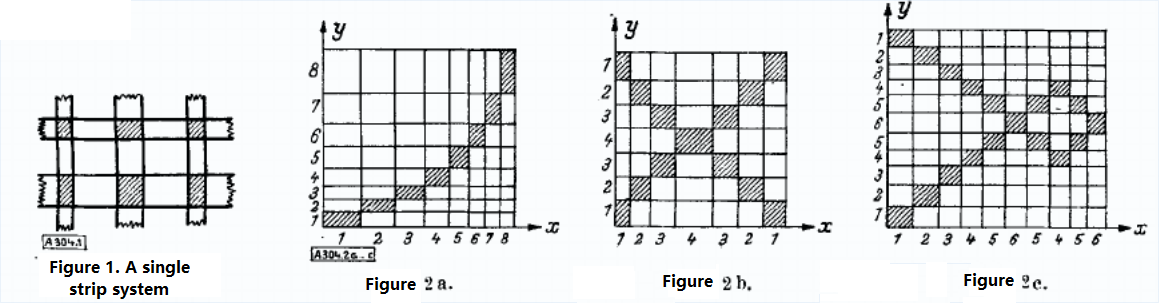
\includegraphics[width=\textwidth]{a.png}
\end{figure}
The figures 2a to c show three examples for such distribution
planes. $w(x,y)$ is non-zero only in the shaded fields,
whose horizontal strip and vertical strip has same number.
If the strip division is infinitely refined, then in the above
observed case, only along 
a curve in the $xy$-plane
that the probability is not zero. The curve is not necessarily a one-to-one correspondence of the $x-$
and $y-$ value, which is assumed in the previous computation
and occurs in the first example of the case. It can also be the curve shown in the other two
examples, which are multi-valued function.
The curve is marked in the distributional plane, in which
there is not a one-to-one relation of $x$ and $y$, but a one-to-one relation for
the $x$-class and $y$-class with the same number.
For the stochastic relation of $x$ and $y$
there exists certain room to move, which is not captured
by the correlation metric $K^2$.

According to the definition of the correlation metric,
$K^2$ does not depend on the specific value of $x$
and $y$ in the distribution.
By now the developed formula of $K^2$ contains explicitly
the function $f(x)$ and $g(y)$ (or only one function).
In particular, we want an expression for the smallest
eigenvalue of the integral equation \eqref{eq:fReducedKernel}.
Such expression does not contain $f(x)$ and
$g(y)$ but only depends on the distribution function
$w(x,y)$.
To obtain such expression, it is suggested to go from \eqref{eq:wxzZero}
which uses double series to expand the kernel
\begin{equation}
        \frac{W(x,z) - w_1(x) w_1(z)}{\sqrt{w_1(x)w_1(z)}}
    = \sum \frac{1}{\lambda_i}
    \sqrt{w_1(x)}f_i(x) \sqrt{w_1(z)}f_i(z) \tag{21}
\end{equation}
We regard the above equation formally and disregard
its convergence and other necessary assumptions.
For $z=x$ the integration about $x$ provides
$$
J = \int \frac{W(x,x) - w_1^2(x)}{w_1(x)} dx
= \frac{1}{\lambda_1}
+ \frac{1}{\lambda_2}
+ \dots
$$
The integrand allows the following two transformations:
$$
\frac{W(x,x) - w_1^2(x)}{w_1(x)}
= \int \frac{w^2(x,y)}{w_1(x)w_2(y)} dy - w_1(x)
=\int \frac{[w(x,y)-w_1(x)w_2(y)]^2}{w_1(x)w_2(y)} dy 
$$
Then it follows for $J$ that
\begin{equation}\label{eq:JlambdaM}
    J=\int \frac{[w(x,y)-w_1(x)w_2(y)]^2}{w_1(x)w_2(y)} dxdy
    = \iint  \frac{w^2(x,y)}{w_1(x)w_2(y)} dxdy-1
    = \frac{1}{\lambda_1}
+ \frac{1}{\lambda_2}
+ \dots
\end{equation}
This expression from its construction coincides with the mean square
contingency of Pearson.
When the first eigenvalue $\lambda_1$
is simple and the series of the reciprocal eigenvalues
converge, it is righteous to solve $\lambda_1$
to show the strength of the correlation.
The two extreme cases do not belong to such situation.
In the full dependence case, $\lambda_i=1$ and $J$
is infinitely large. When this singular behavior
occurs, famous methods from the theory of
integral equation will fail and is not applicable.
A clear and self-understandable result follows when full independence of $x$ and $y$
occurs. $\lambda_1$ is already infinitely large, which
is also true for the remaining eigenvalues. Therefore,
according to \eqref{eq:JlambdaM} $J=0$.

For continuous distributions it is not shown that the value $J$ is a useful
measure of correlation relationship.
But for arithmetic distribution\footnote{For arithmetic distribution
the correlation theory present here can be developed by the elementary
algebra techniques. Such material are introduced thoroughly in the upcoming book about mathematical
statistics. (Publisher Quelle \& Meyer, university education in monograph.)}
there is certain information about the correlation relationship. For arithmetic distribution
the linear equation systems replace the place of integral equation,
and the number of eigenvalues is finite, equal to the row or column
number of the correlation table.

Let $w(x_i, y_k)$
be the probability mass distribution for $m$ possible $x$-values $x_i$
and $n$ possible $y$-values $y_k$, then corresponding to
the kernel function $W(x,z)$ of the integral equation \eqref{eq:fkernel}
we have
$$
W(x_i, x_l)
= \sum_k \frac{w(x_i, y_k) w(x_l, y_k)}{w_2(y_k)}
\textrm{ with } w_2(y_k) = \sum_i w(x_i, y_k)
$$
and the integral equation corresponds to the linear equation system
with $m$ equations.
$$
f(x_i) = \lambda \sum_{l}
\frac{W(x_i, x_l)}{w_1(x_i)} f(x_l)
=\lambda  \sum_{l,k} \frac{w(x_i, y_k) w(x_l, y_k)}{w_1(x_i)w_2(y_k)}
f(x_l).
$$
The trace of the determinant of this equation system is
the sum of all the $m$ reciprocal eigenvalues
$$
\sum_{i,k} \frac{w^2(x_i,y_k)}{w_1(x_i)w_2(y_k)}
= \frac{1}{\lambda_0}
+ \frac{1}{\lambda_1}
+ \dots + \frac{1}{\lambda_{m-1}}.
$$
\end{document}











